%!TEX root = thesis.tex

\chapter{Introduction}
\label{ch:introduction}
\section{What is Pokémon}
\todo{Players move at the same time, unlike in chess.}
\todo{Game states in Pokémon are high-dimensional and the majority of its features are both categorical and partially observable}
\todo{Game is turn based}
\todo{What is a Pokémon? Picture -> Builds (Moveset, ability, item)}

\begin{wrapfigure}{r}{0.5\textwidth}
    \begin{center}
      
\includegraphics[width=0.48\textwidth]{images/pikachu.png}
    \end{center}
    \caption{Pikachu, one of the most popular Pokémon~\autocite{Fandom:AshsPikachu}}
    \label{fig:pikachu-image}
\end{wrapfigure}
Pokémon (an abbreviation for \textbf{Pocket Monsters}) is a media franchise managed my \textit{The Pokémon Company}, a company
founded by \textit{Nintendo}, \textit{Game Freak} and \textit{Creatures}~\autocite{Wikipedia:Pokemon}. Figure \ref{fig:pikachu-image} shows an image of
\textit{Pikachu}, one of the most popular Pokémon. Among multiple movies and series, a large variety of Pokémon games was released, starting with
\textit{Pokémon Red} and \textit{Pokémon Blue} which were released on the 28. September 1998, also known as \ac{GEN1}-games. In order to promote
trading between players, \textit{Nintendo} publishes two very similar games at the same time. 
Both releases differ in a few minor story differences and in the available Pokémon. Therefore, in order to collect all available Pokémon,
players either have to buy two copies of the game or trade with a player that owns the counterpart. As of writing, there are eight major
releases, also called \textit{mainline games} with the latest being \textit{Pokémon Sword} and \textit{Pokémon Shield}. While the graphics
evolved a lot over the years (see figures \ref{fig:red0}, \ref{fig:red1}, \ref{fig:sword0} and \ref{fig:sword1}), the key concept of the 
game remained mostly unchanged.
\begin{figure}[ht]
  \centering
  \begin{minipage}{.5\textwidth}
    \centering
    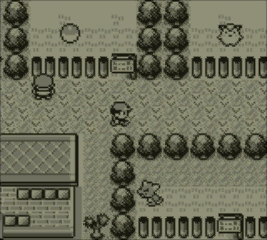
\includegraphics[width=.95\linewidth]{images/Red-0.jpg}
    \captionof{figure}{Exploring the map in \\Pokémon Red}
    \label{fig:red0}
  \end{minipage}%
  \begin{minipage}{.5\textwidth}
    \centering
    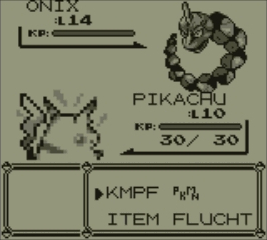
\includegraphics[width=.95\linewidth]{images/Red-1.jpg}
    \captionof{figure}{Fighting another trainer in \\Pokémon Red}
    \label{fig:red1}
  \end{minipage}
  \caption*{Image source: \href{https://www.nintendo.de/Spiele/Game-Boy/Pokemon-Rote-Edition-266109.html}{nintendo.de}}
\end{figure}
The player starts his journey in his hometown to become \textit{Pokémon Champion} which is the highest known 
level of rank for a Pokémon trainer \todo{https://bulbapedia.bulbagarden.net/wiki/Pokémon_Champion}. In order
to achieve this goal, the player has to create a team of up to six individual Pokémon which he then trains 
to unleash their full potential. 
\begin{figure}
  \centering
  \begin{minipage}{.5\textwidth}
    \centering
    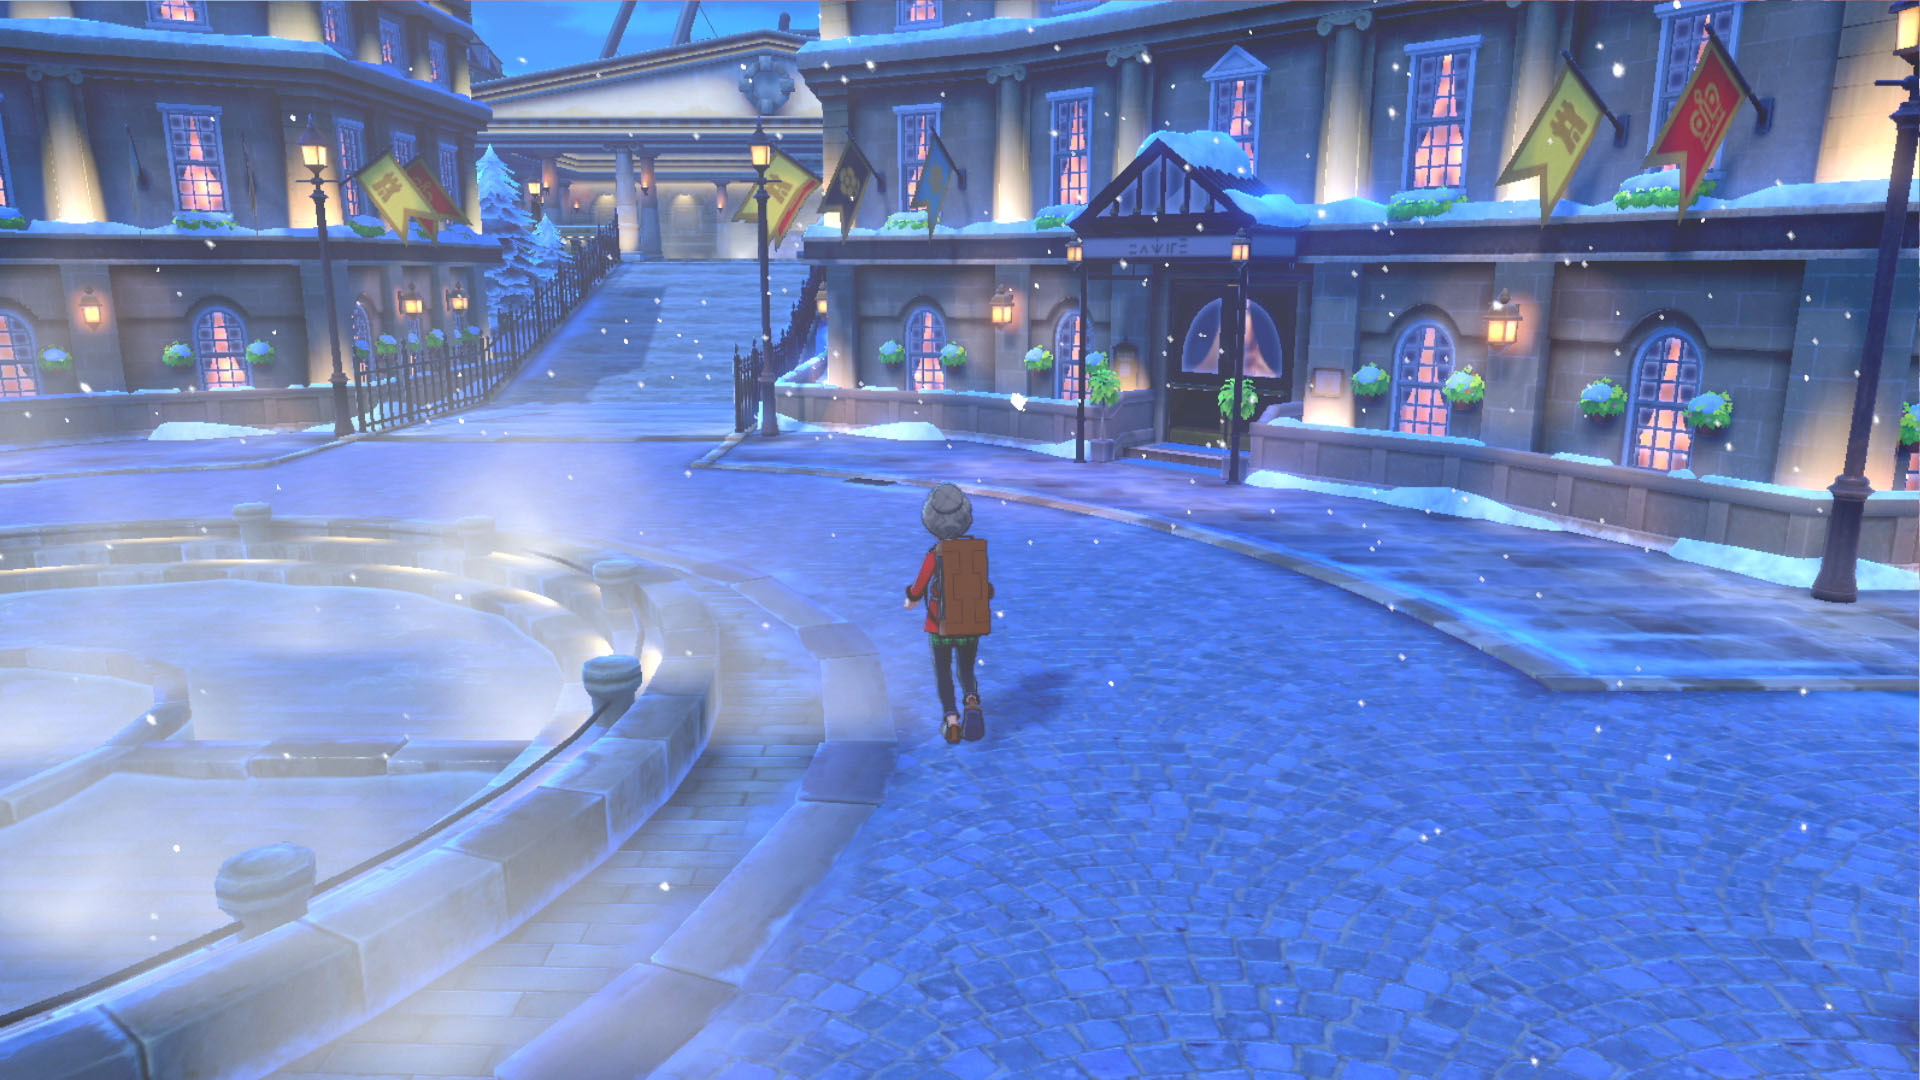
\includegraphics[width=.95\linewidth]{images/Sword-0.jpg}
    \captionof{figure}{Exploring the map in \\Pokémon Sword. \\ 
      Image source: \href{https://swordshield.pokemon.com/de-de/gameplay/pokemon-battle-stadium/}{pokemon.com}}
    \label{fig:sword0}
  \end{minipage}%
  \begin{minipage}{.5\textwidth}
    \centering
    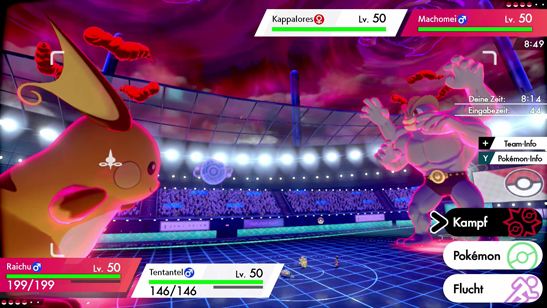
\includegraphics[width=.95\linewidth]{images/Sword-1.jpg}
    \captionof{figure}{Fighting another trainer in \\Pokémon Sword \\
      Image source: \href{https://www.nintendo.de/Spiele/Nintendo-Switch/Pokemon-Schwert-1522111.html}{nintendo.de}}
    \label{fig:sword1}
  \end{minipage}
\end{figure}
This Thesis focuses exclusively on the battling aspect of the game as there are detailed lists of locations and
secrets there is to explore within the games. Pokémon battles are turn based where both players, unlike in 
for example chess, make their decisions at the same time. While the core battle mechanics are very simple, 
the game provides a lot of depth which lead to the formation of a strong competitive battling scene.
\todo{Continue with Showdown}